\chapter{Driven cavity problem}
\begin{figure}[h]
	\centering
	\begin{subfigure}{0.5\textwidth}
		\resizebox{1.4\textwidth}{!}{\input{DrivenCavity/u100}}
		\caption{$Re=100$}
	\end{subfigure}%
	\begin{subfigure}{0.5\textwidth}
		\resizebox{1.4\textwidth}{!}{\input{DrivenCavity/u400}}
		\caption{$Re=400$}
	\end{subfigure}
	\begin{subfigure}{0.5\textwidth}
		\resizebox{1.4\textwidth}{!}{\input{DrivenCavity/u1000}}
		\caption{$Re=1000$}
	\end{subfigure}%
	\begin{subfigure}{0.5\textwidth}
		\resizebox{1.4\textwidth}{!}{\input{DrivenCavity/u3200}}
		\caption{$Re=3200$}
	\end{subfigure}
\end{figure}
\begin{figure}\ContinuedFloat
	\begin{subfigure}{0.5\textwidth}
		\resizebox{1.4\textwidth}{!}{\input{DrivenCavity/u5000}}
		\caption{$Re=5000$}
	\end{subfigure}%
	\begin{subfigure}{0.5\textwidth}
		\resizebox{1.4\textwidth}{!}{\input{DrivenCavity/u7500}}
		\caption{$Re=7500$}
	\end{subfigure}
	\begin{subfigure}{0.5\textwidth}
		\resizebox{1.4\textwidth}{!}{\input{DrivenCavity/u10000}}
		\caption{$Re=10000$}
	\end{subfigure}
	\caption[Comparison between the reference solution and the calculated one of the horizontal velocity along the vertical line in the geometric center of the cavity]{Comparison between the reference solution and the calculated one of the horizontal velocity along the vertical line in the geometric centre of the cavity \cite{Ghia1982}}
\end{figure}

\begin{figure}[H]
	\centering
	\begin{subfigure}{0.5\textwidth}
		\resizebox{1.4\textwidth}{!}{\input{DrivenCavity/v100}}
		\caption{$Re=100$}
	\end{subfigure}%
	\begin{subfigure}{0.5\textwidth}
		\resizebox{1.4\textwidth}{!}{\input{DrivenCavity/v400}}
		\caption{$Re=400$}
	\end{subfigure}
	\begin{subfigure}{0.5\textwidth}
		\resizebox{1.4\textwidth}{!}{\input{DrivenCavity/v1000}}
		\caption{$Re=1000$}
	\end{subfigure}%
	\begin{subfigure}{0.5\textwidth}
		\resizebox{1.4\textwidth}{!}{\input{DrivenCavity/v3200}}
		\caption{$Re=3200$}
	\end{subfigure}
\end{figure}
\begin{figure}\ContinuedFloat
	\begin{subfigure}{0.5\textwidth}
		\resizebox{1.4\textwidth}{!}{\input{DrivenCavity/v5000}}
		\caption{$Re=5000$}
	\end{subfigure}%
	\begin{subfigure}{0.5\textwidth}
		\resizebox{1.4\textwidth}{!}{\input{DrivenCavity/v7500}}
		\caption{$Re=7500$}
	\end{subfigure}
	\begin{subfigure}{0.5\textwidth}
		\resizebox{1.4\textwidth}{!}{\input{DrivenCavity/v10000}}
		\caption{$Re=10000$}
	\end{subfigure}
	\caption[Comparison between the reference solution and the calculated one of the vertical velocity along the horizontal line in the geometric center of the cavity]{Comparison between the reference solution and the calculated one of the vertical velocity along the horizontal line in the geometric centre of the cavity \cite{Ghia1982}}
\end{figure}

\begin{table}[H]
	\centering
	\begin{tabular}{|
			>{\columncolor[HTML]{EFEFEF}}c |c|c|c|c|c|c|c|}
		\hline
		x      & \cellcolor[HTML]{EFEFEF}Re=100 & \cellcolor[HTML]{EFEFEF}Re=400 & \cellcolor[HTML]{EFEFEF}Re=1000 & \cellcolor[HTML]{EFEFEF}Re=3200 & \cellcolor[HTML]{EFEFEF}Re=5000 & \cellcolor[HTML]{EFEFEF}Re=7500 & \cellcolor[HTML]{EFEFEF}Re=10000 \\ \hline
		1      & 0.00\%                         & 0.00\%                         & 0.00\%                          & 0.00\%                          & 0.00\%                          & 0.00\%                          & 0.00\%                           \\ \hline
		0.9766 & 0.53\%                         & 0.41\%                         & 1.07\%                          & 5.91\%                          & 7.13\%                          & 15.08\%                         & 28.11\%                          \\ \hline
		0.9688 & 0.72\%                         & 0.49\%                         & 1.14\%                          & 6.57\%                          & 8.95\%                          & 17.61\%                         & 32.03\%                          \\ \hline
		0.9609 & 1.04\%                         & 0.77\%                         & 1.69\%                          & 7.74\%                          & 10.25\%                         & 18.46\%                         & 33.60\%                          \\ \hline
		0.9531 & 1.32\%                         & 1.06\%                         & 2.40\%                          & 8.22\%                          & 10.50\%                         & 18.68\%                         & 34.58\%                          \\ \hline
		0.8516 & 11.04\%                        & 2.76\%                         & 3.10\%                          & 8.88\%                          & 15.28\%                         & 32.24\%                         & 52.58\%                          \\ \hline
		0.7344 & 1020.07\%                      & 2.66\%                         & 2.01\%                          & 10.68\%                         & 24.81\%                         & 50.19\%                         & 73.70\%                          \\ \hline
		0.6172 & -15.41\%                       & 25.44\%                        & 3.47\%                          & 10.85\%                         & 31.55\%                         & 61.89\%                         & 73.63\%                          \\ \hline
		0.5    & 3.19\%                         & -7.42\%                        & -4.01\%                         & 18.68\%                         & 30.72\%                         & 74.06\%                         & 34.89\%                          \\ \hline
		0.4531 & 7.98\%                         & -5.56\%                        & -1.91\%                         & 91.66\%                         & 30.59\%                         & 64.80\%                         & 112.56\%                         \\ \hline
		0.2813 & 19.18\%                        & 2.53\%                         & 1.24\%                          & 12.55\%                         & 21.26\%                         & 46.49\%                         & 55.93\%                          \\ \hline
		0.1719 & 21.37\%                        & 9.01\%                         & 3.10\%                          & 8.44\%                          & 14.73\%                         & 29.52\%                         & 49.33\%                          \\ \hline
		0.1016 & 20.90\%                        & 12.06\%                        & 5.98\%                          & 5.22\%                          & 8.95\%                          & 17.16\%                         & 36.85\%                          \\ \hline
		0.0703 & 22.33\%                        & 13.08\%                        & 7.10\%                          & 1.78\%                          & 10.75\%                         & 14.22\%                         & 25.13\%                          \\ \hline
		0.0625 & 20.17\%                        & 13.27\%                        & 7.29\%                          & 0.43\%                          & 11.22\%                         & 14.20\%                         & 22.76\%                          \\ \hline
		0.0547 & 19.93\%                        & 13.41\%                        & 7.39\%                          & -1.15\%                         & 11.26\%                         & 13.84\%                         & 20.37\%                          \\ \hline
		0      & 0.00\%                         & 0.00\%                         & 0.00\%                          & 0.00\%                          & 0.00\%                          & 0.00\%                          & 0.00\%                           \\ \hline
	\end{tabular}
	\caption{Error of the horizontal velocities in the vertical central plane}
\end{table}

\begin{table}[H]
	\centering
	\begin{tabular}{|
			>{\columncolor[HTML]{EFEFEF}}c |c|c|c|c|c|c|c|}
		\hline
		y      & \cellcolor[HTML]{EFEFEF}Re=100 & \cellcolor[HTML]{EFEFEF}Re=400 & \cellcolor[HTML]{EFEFEF}Re=1000 & \cellcolor[HTML]{EFEFEF}Re=3200 & \cellcolor[HTML]{EFEFEF}Re=5000 & \cellcolor[HTML]{EFEFEF}Re=7500 & \cellcolor[HTML]{EFEFEF}Re=10000 \\ \hline
		1      & 0.00\%                         & 0.00\%                         & 0.00\%                          & 0.00\%                          & 0.00\%                          & 0.00\%                          & 0.00\%                           \\ \hline
		0.9688 & 7.43\%                         & 2.41\%                         & -1.00\%                         & -1.16\%                         & 11.69\%                         & 17.15\%                         & 20.24\%                          \\ \hline
		0.9609 & 7.29\%                         & 2.02\%                         & -0.95\%                         & 0.95\%                          & 10.81\%                         & 14.42\%                         & 17.89\%                          \\ \hline
		0.9531 & 7.43\%                         & 1.98\%                         & -0.68\%                         & 2.17\%                          & 9.08\%                          & 11.53\%                         & 16.78\%                          \\ \hline
		0.9453 & 7.52\%                         & 1.87\%                         & -0.57\%                         & 3.11\%                          & 7.55\%                          & 10.48\%                         & 18.96\%                          \\ \hline
		0.9063 & 8.21\%                         & -57.88\%                       & 1.57\%                          & 5.68\%                          & 8.89\%                          & 18.94\%                         & 37.44\%                          \\ \hline
		0.8594 & 9.09\%                         & 1.84\%                         & 2.81\%                          & 7.39\%                          & 12.11\%                         & 26.30\%                         & 47.77\%                          \\ \hline
		0.8047 & 10.32\%                        & 1.77\%                         & 3.34\%                          & 9.04\%                          & 16.06\%                         & 35.75\%                         & 53.28\%                          \\ \hline
		0.5    & -6.69\%                        & -14.99\%                       & -10.95\%                        & -40.59\%                        & 3.41\%                          & 61.67\%                         & 331.52\%                         \\ \hline
		0.2344 & 15.90\%                        & 3.89\%                         & 1.56\%                          & 8.54\%                          & 18.07\%                         & 39.01\%                         & 46.30\%                          \\ \hline
		0.2266 & 16.04\%                        & 4.24\%                         & 1.74\%                          & 8.44\%                          & 17.50\%                         & 37.78\%                         & 45.79\%                          \\ \hline
		0.1563 & 16.84\%                        & 6.79\%                         & 3.61\%                          & 6.87\%                          & 12.28\%                         & 26.49\%                         & 44.39\%                          \\ \hline
		0.0938 & 17.15\%                        & 8.22\%                         & 4.96\%                          & 7.54\%                          & 9.99\%                          & 16.36\%                         & 32.74\%                          \\ \hline
		0.0781 & 17.29\%                        & 8.58\%                         & 5.25\%                          & 8.26\%                          & 10.81\%                         & 15.88\%                         & 29.86\%                          \\ \hline
		0.0703 & 17.31\%                        & 8.73\%                         & 5.40\%                          & 8.62\%                          & 11.32\%                         & 16.21\%                         & 29.30\%                          \\ \hline
		0.0625 & 17.29\%                        & 8.82\%                         & 5.51\%                          & 8.93\%                          & 11.70\%                         & 16.66\%                         & 29.23\%                          \\ \hline
		0      & 0.00\%                         & 0.00\%                         & 0.00\%                          & 0.00\%                          & 0.00\%                          & 0.00\%                          & 0.00\%                           \\ \hline
	\end{tabular}
\caption{Error of the vertical velocities in the horizontal central plane}
\end{table}

\section{Horizontal velocities}
\begin{figure}[H]
	\centering
	\begin{subfigure}{0.5\textwidth}
		\resizebox{1.4\textwidth}{!}{\input{DrivenCavity/Ru100}}
		\caption{$Re=100$}
	\end{subfigure}%
	\begin{subfigure}{0.5\textwidth}
		\resizebox{1.4\textwidth}{!}{\input{DrivenCavity/Ru400}}
		\caption{$Re=400$}
	\end{subfigure}
	\begin{subfigure}{0.5\textwidth}
		\resizebox{1.4\textwidth}{!}{\input{DrivenCavity/Ru1000}}
		\caption{$Re=1000$}
	\end{subfigure}%
	\begin{subfigure}{0.5\textwidth}
		\resizebox{1.4\textwidth}{!}{\input{DrivenCavity/Ru3200}}
		\caption{$Re=3200$}
	\end{subfigure}
\end{figure}
\begin{figure}\ContinuedFloat
	\begin{subfigure}{0.5\textwidth}
		\resizebox{1.4\textwidth}{!}{\input{DrivenCavity/Ru5000}}
		\caption{$Re=5000$}
	\end{subfigure}%
	\begin{subfigure}{0.5\textwidth}
		\resizebox{1.4\textwidth}{!}{\input{DrivenCavity/Ru7500}}
		\caption{$Re=7500$}
	\end{subfigure}
	\begin{subfigure}{0.5\textwidth}
		\resizebox{1.4\textwidth}{!}{\input{DrivenCavity/Ru10000}}
		\caption{$Re=10000$}
	\end{subfigure}
	\caption{Horizontal velocity inside the cavity}
\end{figure}

\section{Vertical velocities}
\begin{figure}[H]
	\centering
	\begin{subfigure}{0.5\textwidth}
		\resizebox{1.4\textwidth}{!}{\input{DrivenCavity/Rv100}}
		\caption{$Re=100$}
	\end{subfigure}%
	\begin{subfigure}{0.5\textwidth}
		\resizebox{1.4\textwidth}{!}{% GNUPLOT: LaTeX picture with Postscript
\begingroup
  \makeatletter
  \providecommand\color[2][]{%
    \GenericError{(gnuplot) \space\space\space\@spaces}{%
      Package color not loaded in conjunction with
      terminal option `colourtext'%
    }{See the gnuplot documentation for explanation.%
    }{Either use 'blacktext' in gnuplot or load the package
      color.sty in LaTeX.}%
    \renewcommand\color[2][]{}%
  }%
  \providecommand\includegraphics[2][]{%
    \GenericError{(gnuplot) \space\space\space\@spaces}{%
      Package graphicx or graphics not loaded%
    }{See the gnuplot documentation for explanation.%
    }{The gnuplot epslatex terminal needs graphicx.sty or graphics.sty.}%
    \renewcommand\includegraphics[2][]{}%
  }%
  \providecommand\rotatebox[2]{#2}%
  \@ifundefined{ifGPcolor}{%
    \newif\ifGPcolor
    \GPcolortrue
  }{}%
  \@ifundefined{ifGPblacktext}{%
    \newif\ifGPblacktext
    \GPblacktexttrue
  }{}%
  % define a \g@addto@macro without @ in the name:
  \let\gplgaddtomacro\g@addto@macro
  % define empty templates for all commands taking text:
  \gdef\gplbacktext{}%
  \gdef\gplfronttext{}%
  \makeatother
  \ifGPblacktext
    % no textcolor at all
    \def\colorrgb#1{}%
    \def\colorgray#1{}%
  \else
    % gray or color?
    \ifGPcolor
      \def\colorrgb#1{\color[rgb]{#1}}%
      \def\colorgray#1{\color[gray]{#1}}%
      \expandafter\def\csname LTw\endcsname{\color{white}}%
      \expandafter\def\csname LTb\endcsname{\color{black}}%
      \expandafter\def\csname LTa\endcsname{\color{black}}%
      \expandafter\def\csname LT0\endcsname{\color[rgb]{1,0,0}}%
      \expandafter\def\csname LT1\endcsname{\color[rgb]{0,1,0}}%
      \expandafter\def\csname LT2\endcsname{\color[rgb]{0,0,1}}%
      \expandafter\def\csname LT3\endcsname{\color[rgb]{1,0,1}}%
      \expandafter\def\csname LT4\endcsname{\color[rgb]{0,1,1}}%
      \expandafter\def\csname LT5\endcsname{\color[rgb]{1,1,0}}%
      \expandafter\def\csname LT6\endcsname{\color[rgb]{0,0,0}}%
      \expandafter\def\csname LT7\endcsname{\color[rgb]{1,0.3,0}}%
      \expandafter\def\csname LT8\endcsname{\color[rgb]{0.5,0.5,0.5}}%
    \else
      % gray
      \def\colorrgb#1{\color{black}}%
      \def\colorgray#1{\color[gray]{#1}}%
      \expandafter\def\csname LTw\endcsname{\color{white}}%
      \expandafter\def\csname LTb\endcsname{\color{black}}%
      \expandafter\def\csname LTa\endcsname{\color{black}}%
      \expandafter\def\csname LT0\endcsname{\color{black}}%
      \expandafter\def\csname LT1\endcsname{\color{black}}%
      \expandafter\def\csname LT2\endcsname{\color{black}}%
      \expandafter\def\csname LT3\endcsname{\color{black}}%
      \expandafter\def\csname LT4\endcsname{\color{black}}%
      \expandafter\def\csname LT5\endcsname{\color{black}}%
      \expandafter\def\csname LT6\endcsname{\color{black}}%
      \expandafter\def\csname LT7\endcsname{\color{black}}%
      \expandafter\def\csname LT8\endcsname{\color{black}}%
    \fi
  \fi
    \setlength{\unitlength}{0.0500bp}%
    \ifx\gptboxheight\undefined%
      \newlength{\gptboxheight}%
      \newlength{\gptboxwidth}%
      \newsavebox{\gptboxtext}%
    \fi%
    \setlength{\fboxrule}{0.5pt}%
    \setlength{\fboxsep}{1pt}%
\begin{picture}(7200.00,5040.00)%
    \gplgaddtomacro\gplbacktext{%
    }%
    \gplgaddtomacro\gplfronttext{%
      \put(1908,624){\makebox(0,0){\strut{}$0$}}%
      \put(2585,624){\makebox(0,0){\strut{}$0.2$}}%
      \put(3262,624){\makebox(0,0){\strut{}$0.4$}}%
      \put(3938,624){\makebox(0,0){\strut{}$0.6$}}%
      \put(4615,624){\makebox(0,0){\strut{}$0.8$}}%
      \put(5292,624){\makebox(0,0){\strut{}$1$}}%
      \put(1720,938){\makebox(0,0)[r]{\strut{}$0$}}%
      \put(1720,1615){\makebox(0,0)[r]{\strut{}$0.2$}}%
      \put(1720,2292){\makebox(0,0)[r]{\strut{}$0.4$}}%
      \put(1720,2968){\makebox(0,0)[r]{\strut{}$0.6$}}%
      \put(1720,3645){\makebox(0,0)[r]{\strut{}$0.8$}}%
      \put(1720,4322){\makebox(0,0)[r]{\strut{}$1$}}%
      \put(5678,938){\makebox(0,0)[l]{\strut{}$-0.7$}}%
      \put(5678,1245){\makebox(0,0)[l]{\strut{}$-0.6$}}%
      \put(5678,1553){\makebox(0,0)[l]{\strut{}$-0.5$}}%
      \put(5678,1860){\makebox(0,0)[l]{\strut{}$-0.4$}}%
      \put(5678,2168){\makebox(0,0)[l]{\strut{}$-0.3$}}%
      \put(5678,2476){\makebox(0,0)[l]{\strut{}$-0.2$}}%
      \put(5678,2783){\makebox(0,0)[l]{\strut{}$-0.1$}}%
      \put(5678,3091){\makebox(0,0)[l]{\strut{}$0$}}%
      \put(5678,3399){\makebox(0,0)[l]{\strut{}$0.1$}}%
      \put(5678,3706){\makebox(0,0)[l]{\strut{}$0.2$}}%
      \put(5678,4014){\makebox(0,0)[l]{\strut{}$0.3$}}%
      \put(5678,4322){\makebox(0,0)[l]{\strut{}$0.4$}}%
    }%
    \gplbacktext
    \put(0,0){\includegraphics{DrivenCavity/Rv400}}%
    \gplfronttext
  \end{picture}%
\endgroup
}
		\caption{$Re=400$}
	\end{subfigure}
	\begin{subfigure}{0.5\textwidth}
		\resizebox{1.4\textwidth}{!}{\input{DrivenCavity/Rv1000}}
		\caption{$Re=1000$}
	\end{subfigure}%
	\begin{subfigure}{0.5\textwidth}
		\resizebox{1.4\textwidth}{!}{\input{DrivenCavity/Rv3200}}
		\caption{$Re=3200$}
	\end{subfigure}
\end{figure}
\begin{figure}\ContinuedFloat
	\begin{subfigure}{0.5\textwidth}
		\resizebox{1.4\textwidth}{!}{\input{DrivenCavity/Rv5000}}
		\caption{$Re=5000$}
	\end{subfigure}%
	\begin{subfigure}{0.5\textwidth}
		\resizebox{1.4\textwidth}{!}{\input{DrivenCavity/Rv7500}}
		\caption{$Re=7500$}
	\end{subfigure}
	\begin{subfigure}{0.5\textwidth}
		\resizebox{1.4\textwidth}{!}{\input{DrivenCavity/Rv10000}}
		\caption{$Re=10000$}
	\end{subfigure}
	\caption{Vertical velocity inside the cavity}
\end{figure}

\section{Streamlines}
\begin{figure}[H]
	\centering
	\begin{subfigure}{0.5\textwidth}
		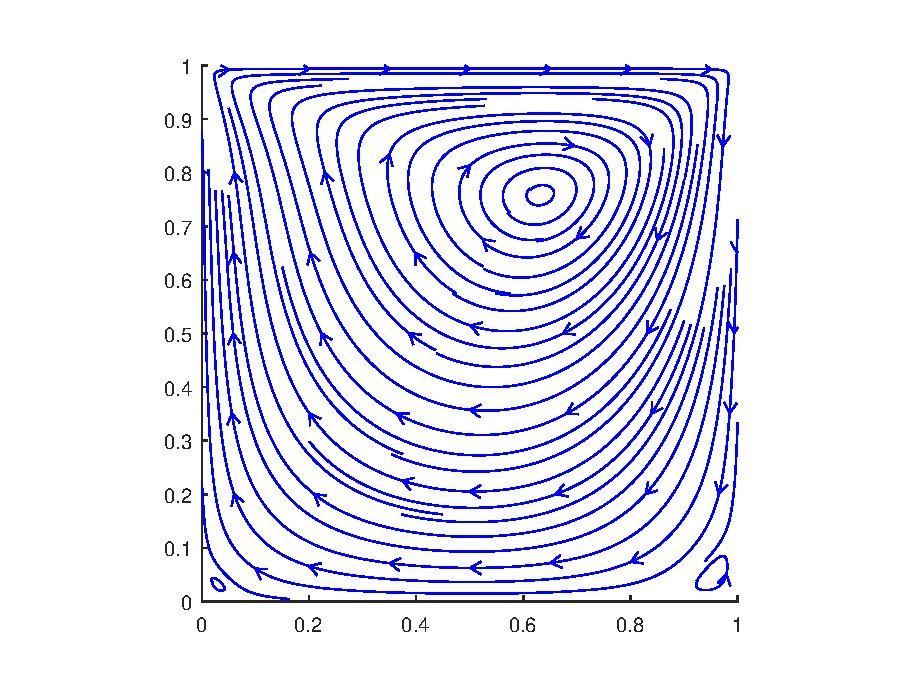
\includegraphics[scale=0.61]{DrivenCavity/100}
		\caption{$Re=100$}
	\end{subfigure}%
	\begin{subfigure}{0.5\textwidth}
		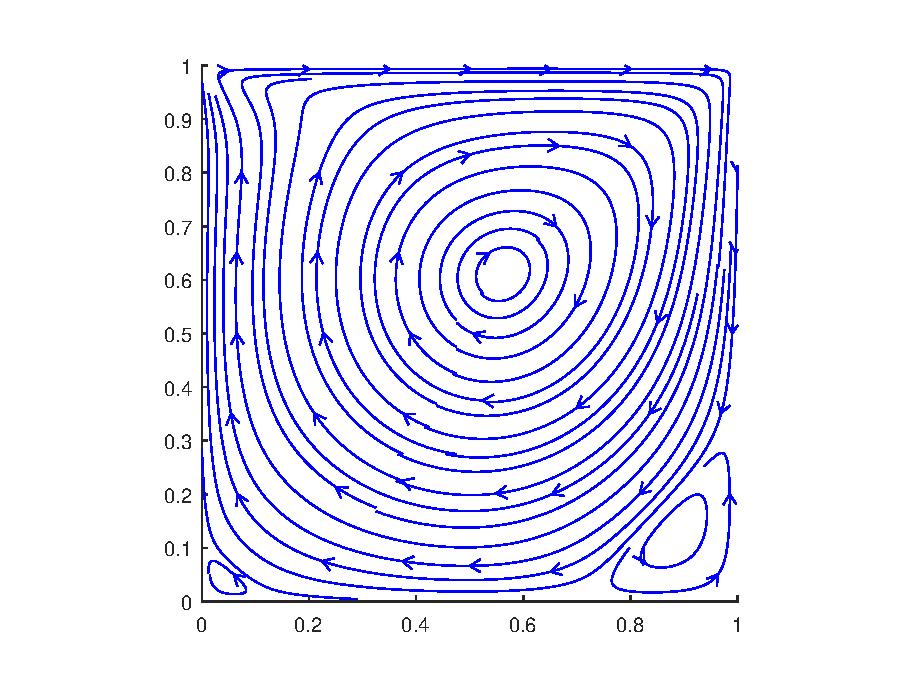
\includegraphics[scale=0.61]{DrivenCavity/400}
		\caption{$Re=400$}
	\end{subfigure}
	\begin{subfigure}{0.5\textwidth}
		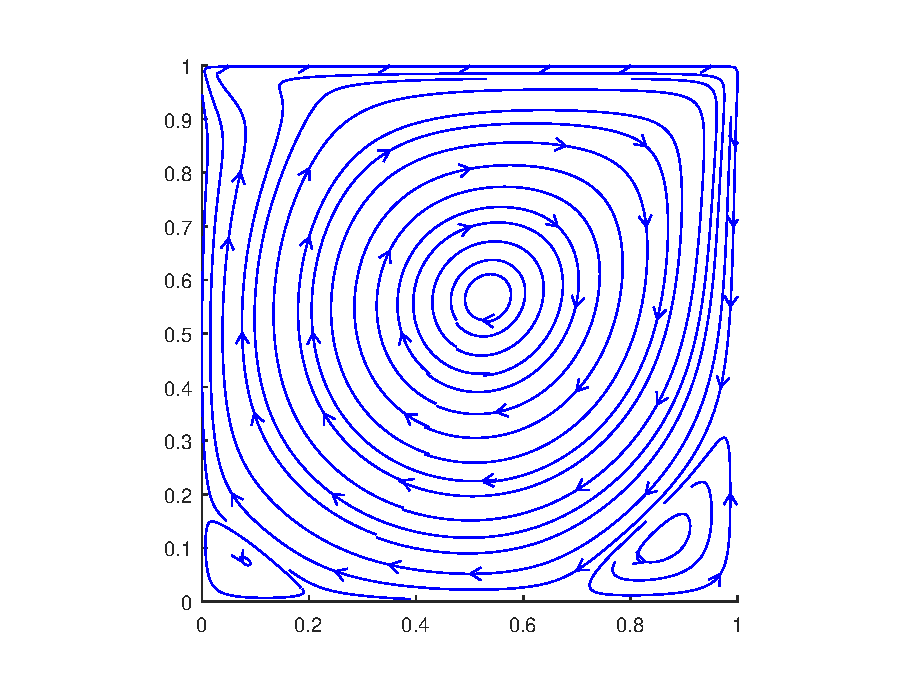
\includegraphics[scale=0.61]{DrivenCavity/1000}
		\caption{$Re=1000$}
	\end{subfigure}%
	\begin{subfigure}{0.5\textwidth}
		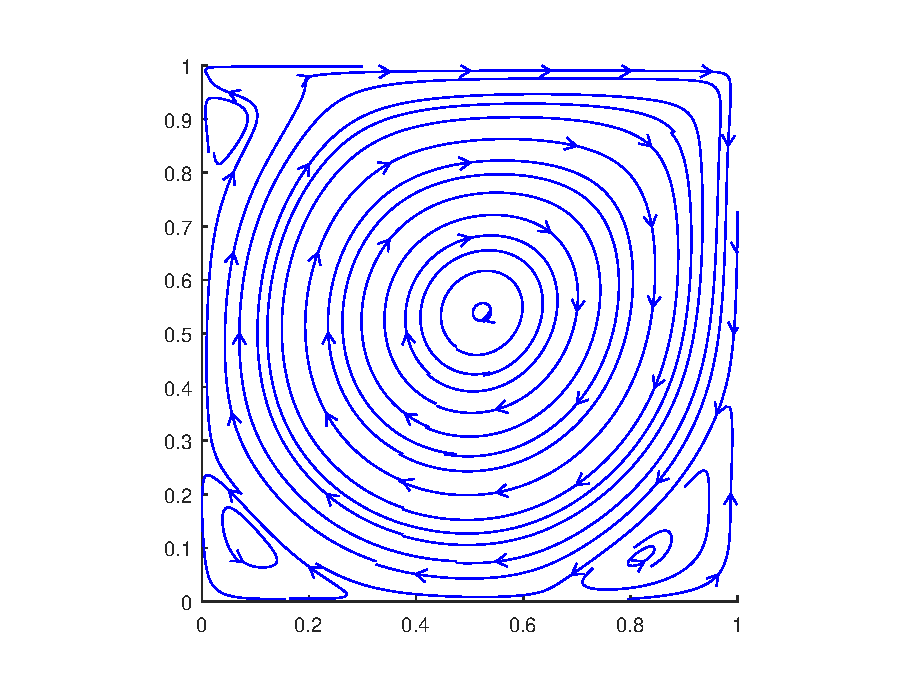
\includegraphics[scale=0.61]{DrivenCavity/3200}
		\caption{$Re=3200$}
	\end{subfigure}
\end{figure}
\begin{figure}\ContinuedFloat
	\begin{subfigure}{0.5\textwidth}
		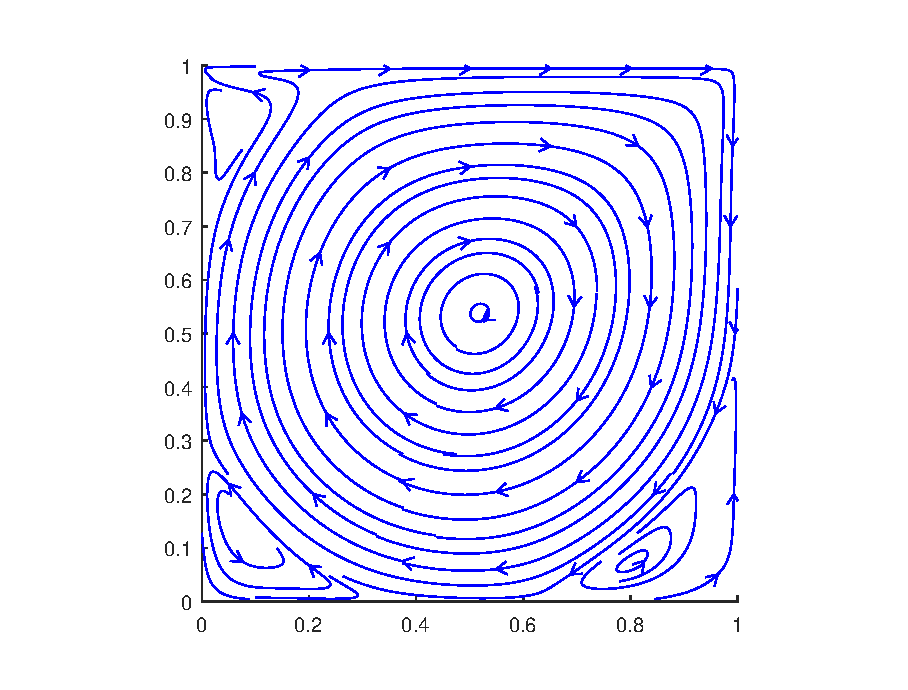
\includegraphics[scale=0.61]{DrivenCavity/5000}
		\caption{$Re=5000$}
	\end{subfigure}%
	\begin{subfigure}{0.5\textwidth}
		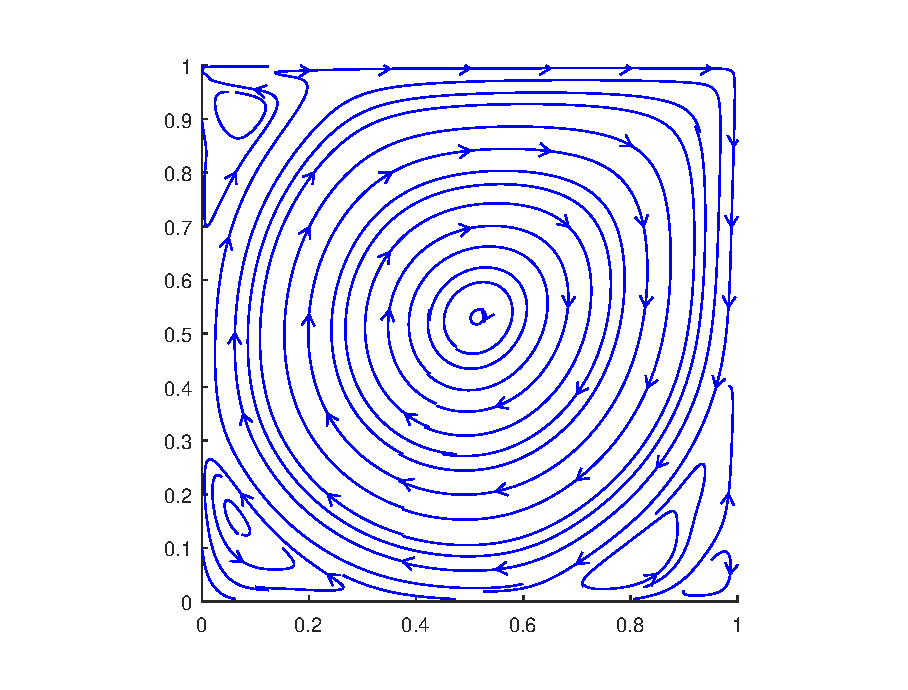
\includegraphics[scale=0.61]{DrivenCavity/7500}
		\caption{$Re=7500$}
	\end{subfigure}
	\begin{subfigure}{0.5\textwidth}
		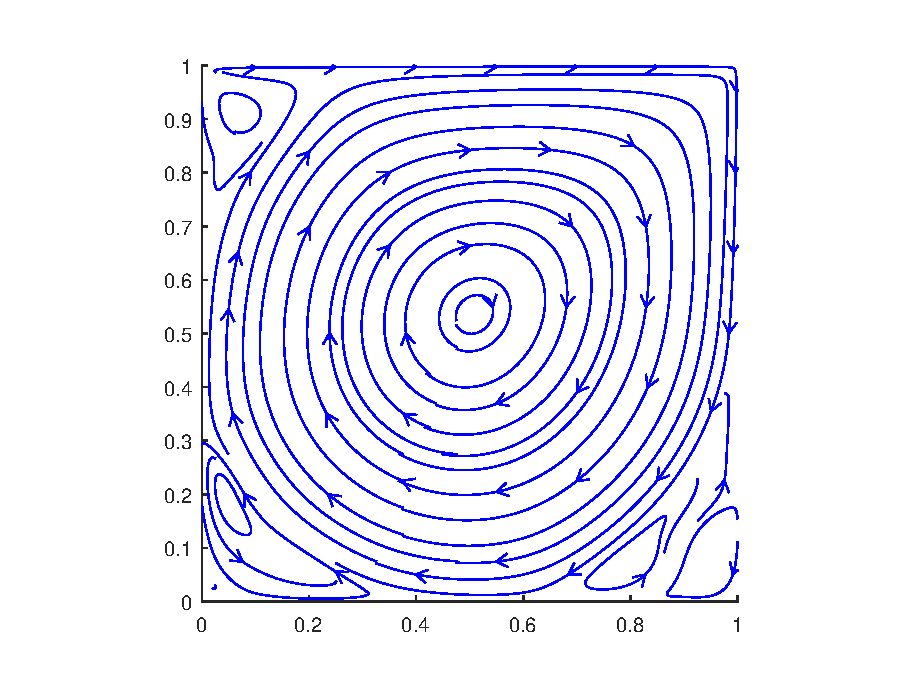
\includegraphics[scale=0.61]{DrivenCavity/10000}
		\caption{$Re=10000$}
	\end{subfigure}
	\caption{Streamlines of the flow inside the cavity}
\end{figure}